\section*{Detecting Sinusoids}

Before we attempt to transform a time domain signal to the frequency domain, we will need to solve
a simpler problem.  Let us first try and develop a tool to detect whether a particular frequency/sinusoid 
is present in some sequence of audio samples. Figure 
\ref{fig:test} shows a diagram of such a testing device.  It should be able to take our signal and some frequency
and output one of two options: yes, the frequency is part of the signal or no, the frequency is not part of the signal.
If we can do that, we can test our samples against
a whole range of frequencies, allowing us to construct a good sketch of the frequency domain.   In essence,
 this is the approach of the DFT, and the testing device we use to detect frequencies is called the ``inner product".
 
 \begin{figure}[h]
 	\caption{A sketch of the desired procedure for determining frequency in a signal.}
 	\centering
 	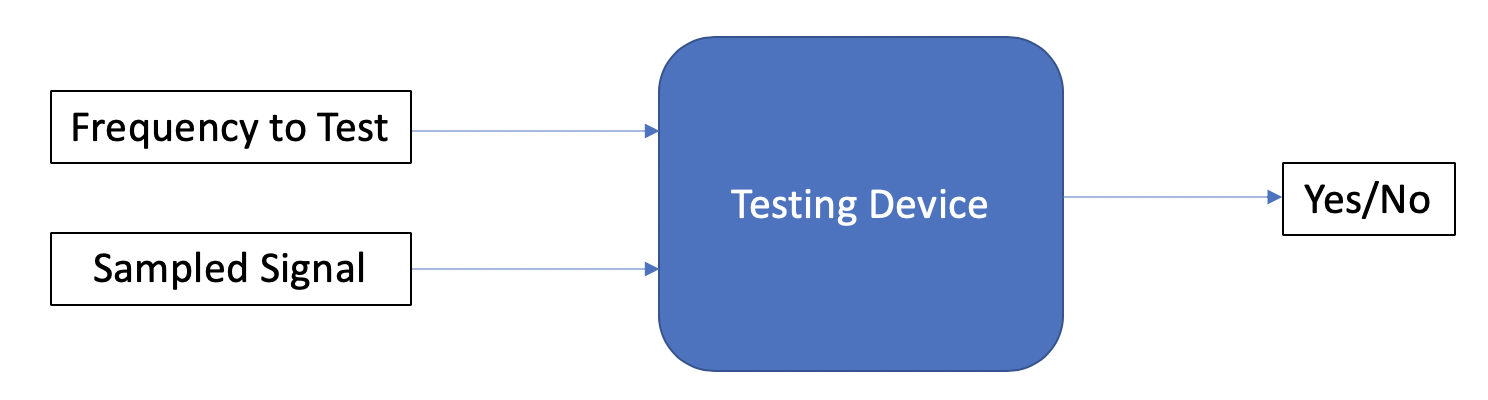
\includegraphics[scale = 0.4]{test.png}
 	\label{fig:test}
 \end{figure}

\subsection*{Orthogonality and the Inner Product}

The inner product is an operation just like addition or multiplication and has several definitions depending
upon the application.  Unlike addition and multiplication, the inputs to the inner product are not numbers, but \textbf{sequences} of numbers.
What exactly is a sequence of numbers?  A sequence
is simply an ordered collection.  In digital signal 
processing, a sequence of numbers is defined with square brackets.  For example, we could have a sequence
$[9, -2, 7]$.  Because sequences are ordered, the sequence $[9, -2, 7]$ is distinct from $[-2, 7, 9]$.  It matters
that the initial element is $9$ rather than $-2$.  

Additionally, we like to give sequences names so that we can easily refer to them.  
We could assign the sequence $[9, -2, 7]$ the name $x$ with an index variable $n$ such that 
$x[n] = [9, -2, 7]$.  The index variable is used to refer to any element in the sequence.  For example,
the notation $x[0]$ refers to the zeroth element in the sequence, namely 9.  In digital signal processing
and nearly all computer languages, we always number sequences starting with index zero.  It can
be a confusing convention at first.  For example, $x[1]$ refers to $-2$ and not $9$.  In digital signal processing,
sequences generally hold samples of audio (i.e., amplitudes).  So a sequence like $x[n] = [0.5, 0.2, 0]$ is a sound file with three samples of amplitude 0.5, 0.2, and 0.

Sequences are the inputs to the inner product.  \textbf{The inner product is calculated by multiplying
the values at each index of the two sequences and then summing those products}.  Note that the length of
each sequence must be the same.  As an example, let us
take two sequences: $x[n] = [1, 2, 3]$ and $y[n] = [1, -1, 0]$.  The inner product of $x[n]$ and $y[n]$ is $(1 * 1) + (2 * -1) + (3 * 0) = -1$.
We take the first numbers of each sequence and multiply them.  Then we multiply the second
numbers and then the third numbers and add them all up.  In this example, that sum is -1.  The inner product 
will always yield a single number.  If the result is zero, we say that the two sequences are
orthogonal.  In this case, $x$ and $y$ are not orthogonal because the result is $-1$.  
In math, we often use angle brackets to denote
the inner product.  For example, the inner product of sequences $x$ and $y$ is notated as $\langle x, y \rangle$.

\begin{figure}[h]
	\caption{Two sinusoids that are periodic along the interval 0 to $L$.}
	\centering
	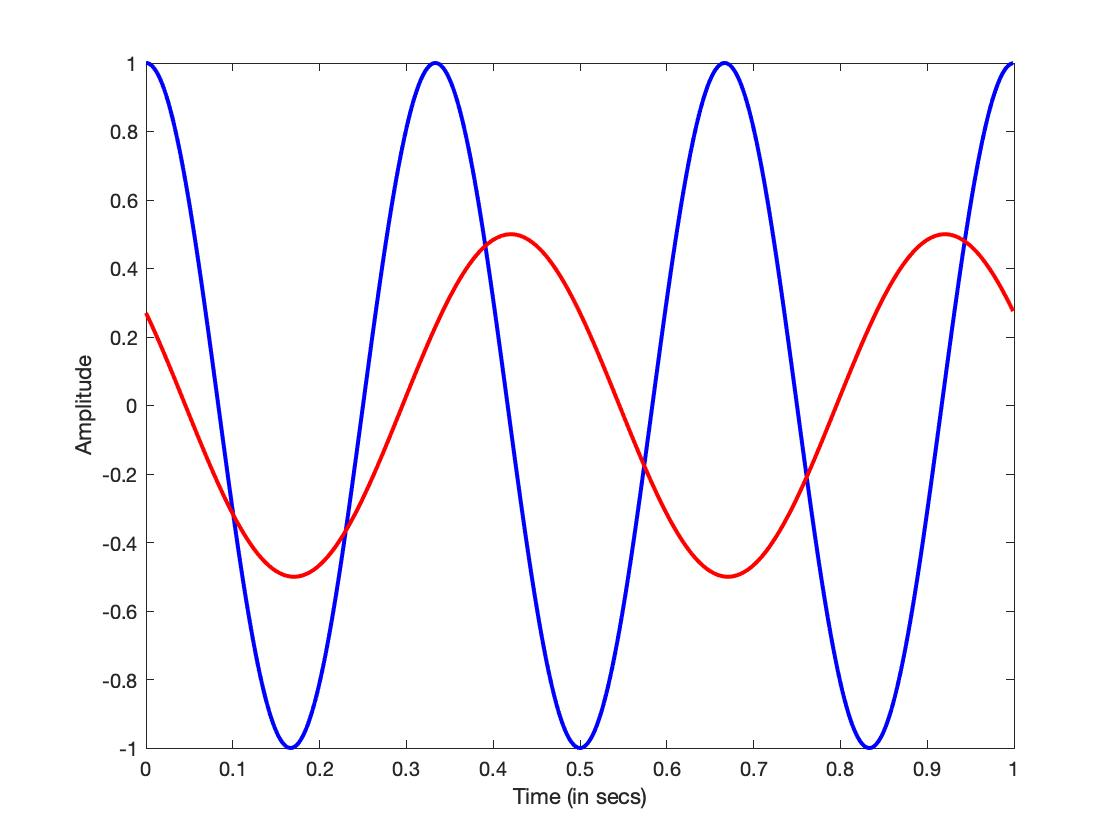
\includegraphics[scale = 0.3]{twoSinusoids.jpg}
	\label{fig:twoSines}
\end{figure}

%We can also take the inner product of two functions as well.  The inner product for two functions is also defined
%as the sum of pointwise products.  Consider the two sinusoids shown in Figure \ref{fig:twoSines}.  The red 
%wave can be expressed as $0.5\cos(2\pi(2)t + 1)$, and the blue wave 
%can be expressed as $\sin(2\pi(3)t + \pi/2)$.  In this example, we will take the inner product over a specific 
%range of time from $t = 0$ to $t = 1$.  To begin, we start with
%the first points from the red and blue sinusoids at $t = 0$.
%At that moment, the red sinusoid has an amplitude of about 0.25 and the blue sinusoid has
%an amplitude of 1.0.  The product of these two values would be $1.0 * 0.25 = 0.25$.  That constitutes the first pointwise product.
%To calculate the sum of all the other pointwise products, we would need to do this same procedure for every value of $t$ between 0 and 1.  That's an infinite number of points!  Fortunately, 
%if we can express these sinusoids in the form $A\sin(2\pi ft + \phi)$, then
%the calculation becomes relatively trivial with calculus.  The inner product for these two functions over this time 
%period is zero,
%and therefore the functions are orthogonal over that time period.

It is important to note that we have not proven anything or ascribed any significance yet to the inner product
or orthogonality.  We have simply defined an operation (i.e, the inner product) that can be performed on any two sequences,
nothing more.  Similarly, orthogonality is simply a label attached to the result of the inner product if it is zero.  
So why do we care about orthogonality and the inner product?  It turns out that orthogonality and 
sinusoids have an important 
mathematical relationship.  If we take two sequences representing any two sinusoids and take their inner product, 
the result is zero
(i.e., orthogonal) 
\textbf{except when the two sinusoids have the same frequency}.  This simple property is the key to 
understanding how the DFT works.  Note that there are some caveats to this claim that we will discuss soon.

Any two sinusoids of different frequencies are orthogonal no matter their phase or amplitude.  A key caveat though
is that the sequences for each sinusoid must represent an integer number of periods.  
In other words, the sinusoids must be periodic along the time represented by the samples in the sequence.  
This is a crucial point and one that 
will be paramount for 
understanding the limitations of the Discrete Fourier Transform.  For example, Figure \ref{fig:twoSines} depicts two periodic sinusoids.
How do we know they are periodic?  Because both the blue and the red sinusoids start and end at the same place in their respective curve.  Each of them completes an integer numbers of cycles.  

Let us show that these two sinusoids are orthogonal by generating a sequence of samples for each sinusoid. Recall 
that the inner product takes sequences as input.  If you look at Figure \ref{fig:twoSines}, we can see that the red sinusoid
completes two complete cycles over a period of 1 second.  Therefore, it has a frequency of 2Hz.  The blue sinusoid
completes three full cycles so it has a frequency of 3Hz.  We should expect that when we take the inner product
of these two sequences of samples that we get a result of zero because the frequencies are different.  
To start, we need to choose a sampling rate that will prevent aliasing.  Anything above 6Hz will suffice, so for ease let us
 choose 8 Hz.  Figure \ref{fig:twoSinesPoints} shows 
where those samples lie on our two sinusoids.  The samples for the blue sinusoid are approximately $b[n] = [1, -0.707, 0, 0.707, -1, 0.707, 0, -0.707]$ and the samples for the red
sinusoid are $r[n] = [0.27, -0.421, -0.27, 0.421, 0.27, -0.421, -0.27, 0.421]$.  The inner
product of $b[n]$ and $r[n]$ is equal to (1 * 0.27) + (-0.707 * -0.421) + (0 * -0.27) + 
(0.707 * 0.421) + (-1 * 0.27) + (0.707 * -0.421) + (0 * -0.27) + (-0.707 * 0.421) = 0.  Indeed these sequences are orthogonal, which is expected because the two sinusoids have different frequencies.

\begin{figure}[h]
	\caption{Two sinusoids that are periodic along the interval 0 to $L = 1$.}
	\centering
	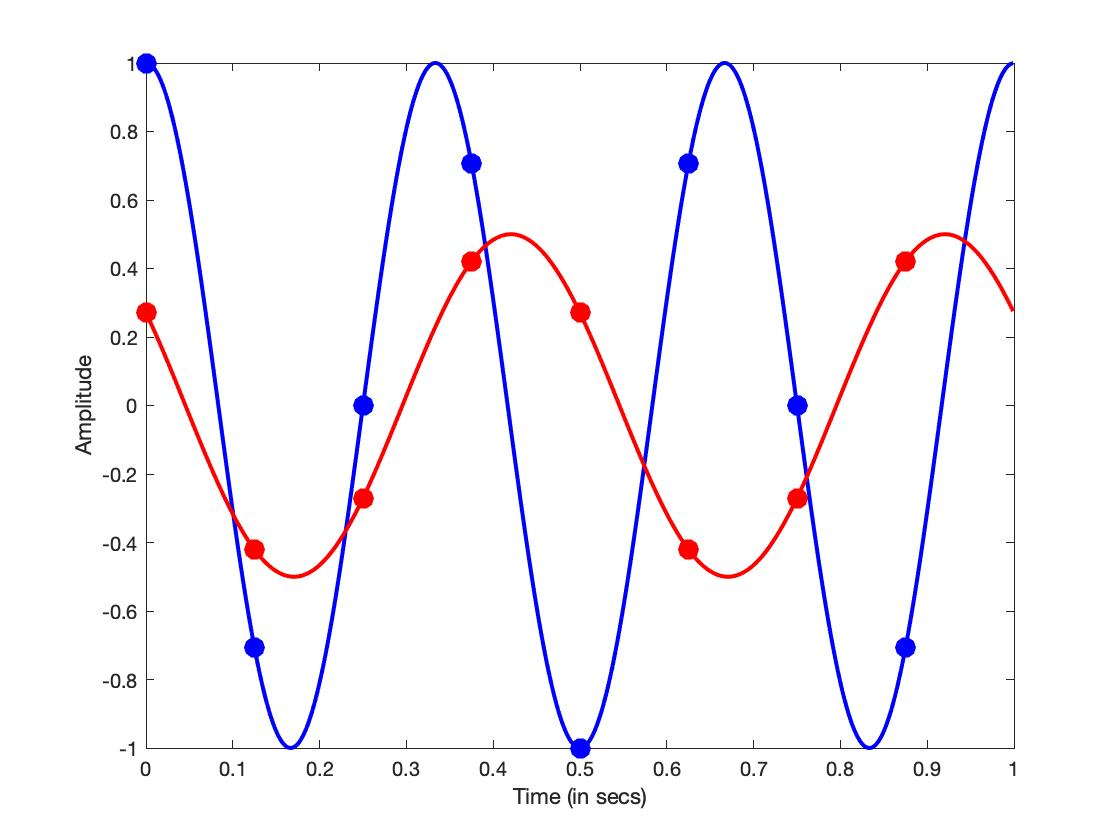
\includegraphics[scale = 0.3]{twoSinusoidsPoints.jpg}
	\label{fig:twoSinesPoints}
\end{figure}

As a side note, samples for a sinusoid $A\sin(2\pi ft + \phi)$ can be generated by replacing time 
$t$ with $Tn$ where $T$ is
the sampling period and $n$ is the sample number or index.  $T$ is related to the sampling rate $f_s$.
$T$ specifies the amount of time between each sample and can be calculated as $1/f_s$.  The two
sequences $b[n]$ and $r[n]$ were generated by sampling the sinusoids $\sin(6\pi t + \pi/2)$ and
$0.5\cos(4\pi t + 1)$.  Therefore, $b[n] = \sin(6\pi Tn + \pi/2)$ and $r[n] = 0.5\cos(4\pi Tn + 1)$.

Let us briefly summarize the conditions when two sinusoids of different frequencies
are orthogonal:

\begin{itemize}
	\item the two sinusoids are both periodic along the time interval spanned by the sequences
	\item if sampled, the sample rate is greater than twice the frequency of both sinusoids
\end{itemize}

\textbf{Moving forward unless otherwise indicated, our 
claims will always be based on these two assumptions even when not explicitly indicated.}

\subsection*{Probing for Sinusoids}

As stated at the beginning of this section, the inner product will be our tool for
detecting frequencies in an audio signal.  To this point, we have seen how the inner
product of two sinusoids can determine the similarity of their frequencies.  If the result
of the inner product is non-zero, we know the sinusoids must have the same frequency.
If the result is zero (i.e., orthogonal), the sinusoids must have different frequencies.  Note that
there is one more caveat left to discuss with the latter conclusion that we will address shortly.

Unfortunately, most audio signals are not a single sinusoid.  So how can the inner product 
detect the presence of sinusoids in a more complex audio signal?
Recall that any song, speech, soundscape, or any other kind of audio can be broken down into a sum of 
sinusoids as shown below.

$$A_1\sin(2\pi f_1 t + \phi_1) + A_2\sin(2 \pi f_2 t + \phi_2) + A_3\sin(2 \pi f_3 t + \phi_3) + ...$$

\noindent The inner product has a special property called the \textbf{distributive property}.
The term ``distributive" in mathematics applies
to many different operations.  For example, we know from alebgra that the distributive property of 
multiplication over addition means that $x * (y + z) = x * y + x * z$.  We see that the multiplication operator can apply
to each individual component and the result is just the same.  The same is true for the inner product!\footnote{
	We will not spend any time proving this truth here.  But it is actually not too difficult to do so.  
	The inner product is simply a series of multiplications and additions.  So with some clever rearranging of terms, 
	we can show that the distributive property is true for inner products.
}
If we have any sequence $x$ and any other
sequence composed of sequences $y$ and $z$, then the distributive property for inner products 
means that  $\langle x, y + z \rangle = \langle x, y \rangle + \langle x, z \rangle$.  

 We know now that when the inner product of some test frequency is 
applied to some arbitrary signal composed of sinusoids, the result is equivalent to the inner product of
our test frequency with each sinusoidal component.  We just analyzed the meaning of the inner product
of two sinusoids.  Anything that is non-zero means that two sinusoids are the same frequency.  Orthogonality
 means the two sinusoids are of different frequency.  Therefore, a non-zero result
indicates that the frequency is a part of that
signal.  A result of zero means that the frequency is not a part of the signal.  So the inner product
is our tool to implement Figure \ref{fig:test}.  

To solidify this concept, let us take eight samples from some signal and test that signal for certain
frequencies.  We will name the signal $x[n]$ and we will assume that the sampling rate is 8Hz.  Here
are those samples:

$$x[n] = [0.1728, 0.2574, -0.0445, -0.0432, -0.1728, -0.2574, 0.0445, 0.0432]$$

\noindent Let us first test to see whether 2Hz is present in the signal.  To do so, let us generate samples
from a 2Hz sinusoid.  Here are those samples below set to the variable $t$:

$$t[n] = [0, 1, 0, -1, 0, 1, 0, -1]$$

\noindent Let us now take the inner product of $x[n]$ with $t[n]$, notated as $\langle x, t \rangle$.

$$\langle x, t \rangle = (0.1728 \cdot 0) + (0.2574 \cdot 1) + (-0.0445 \cdot 0) + ... = 0$$

\noindent The result of the inner product of $x$ and $t$ is zero, meaning that $x$ and $t$ are orthogonal.  Therefore,
the frequency 2Hz is not part of the audio signal $x$.  

Let us test another frequency.  Let us generate samples for 3Hz to see if that frequency is present in $x$.  
Below are samples from a 3Hz sine wave.

$$u[n] = [0, 0.7071, -1, 0.7071, 0, -0.7071, 1, -0.7071]$$

\noindent Again let us take the inner product of $x$ with $u$.  This time the result is 0.392.  A non-zero
result indicates that 3Hz is present in $x$.  We could test $x$ against other frequencies to see if they exist.  
The samples for $x$ were generated from the following function $0.2\sin(2\pi t + 1.3) + 0.1\sin(6\pi t -0.2)$.
As you can see 3Hz is represented by $0.1\sin(6\pi t -0.2)$.  If we tested $x$ against a frequency of 1Hz, we
would also get a non-zero result.

As an important reminder, orthogonality of sinusoids is predicated on the fact that all sinsuoids are periodic
along the same interval.  In this somewhat contrived example, I was careful to assemble a signal $x$ whose
frequency components were periodic along one second of time.  This limited the creation of $x$ to only
integer frequencies.  Similarly, I made sure to test $x$ only with integer frequencies as well.  Suppose I tested
$x$ against the samples of a frequency like 1.5Hz.  We would get a non-zero inner product!  This would seem
to indicate the presence of 1.5Hz in the signal even though $x$ was derived only from a sinusoid of 1Hz
and 3Hz.  The issue is that 1.5Hz is \textbf{not} periodic across a time period of one second.  It is paramount
to remember that all of the claims made so far are based upon the critical restriction that both the testing sinusoid
and the components of our audio signal are all periodic along the same distance.  Later in this document,
we will return to the issue of aperiodicity but for now our claims will be based on this assumption.

\subsection*{The Pesky $\pi/2$ Problem}

It seems as though we have solved the problem stated at the outset of this section.  We have discovered a tool
that can detect the presence of a single frequency in any audio signal by taking the inner product of the signal
and a sinusoid with some testing frequency.  And essentially we have, but there is one special caveat that
we need to address.  \textbf{It is not true that only sinusoids of different frequencies are orthogonal.  Two sinusoids of the same frequency are also orthogonal when their phase differs by $\pi/2$.}  

Why is this problematic?  The inner product was supposed to be our perfect tool that could definitively determine
the presence of a sinusoid.  If the result was non-zero, the sinusoids have the same frequency.  If the result was
zero, the sinsusoids have different frequencies.  The former is still true but the latter may not always be.  It is 
possible that we could take the inner product of some audio signal against a testing sinusoid and get a result
of zero even when the testing frequency is part of the audio signal.  

\begin{figure}[h]
	\caption{A depiction of the result and its meaning from the inner product of a signal and a testing frequency}
	\centering
	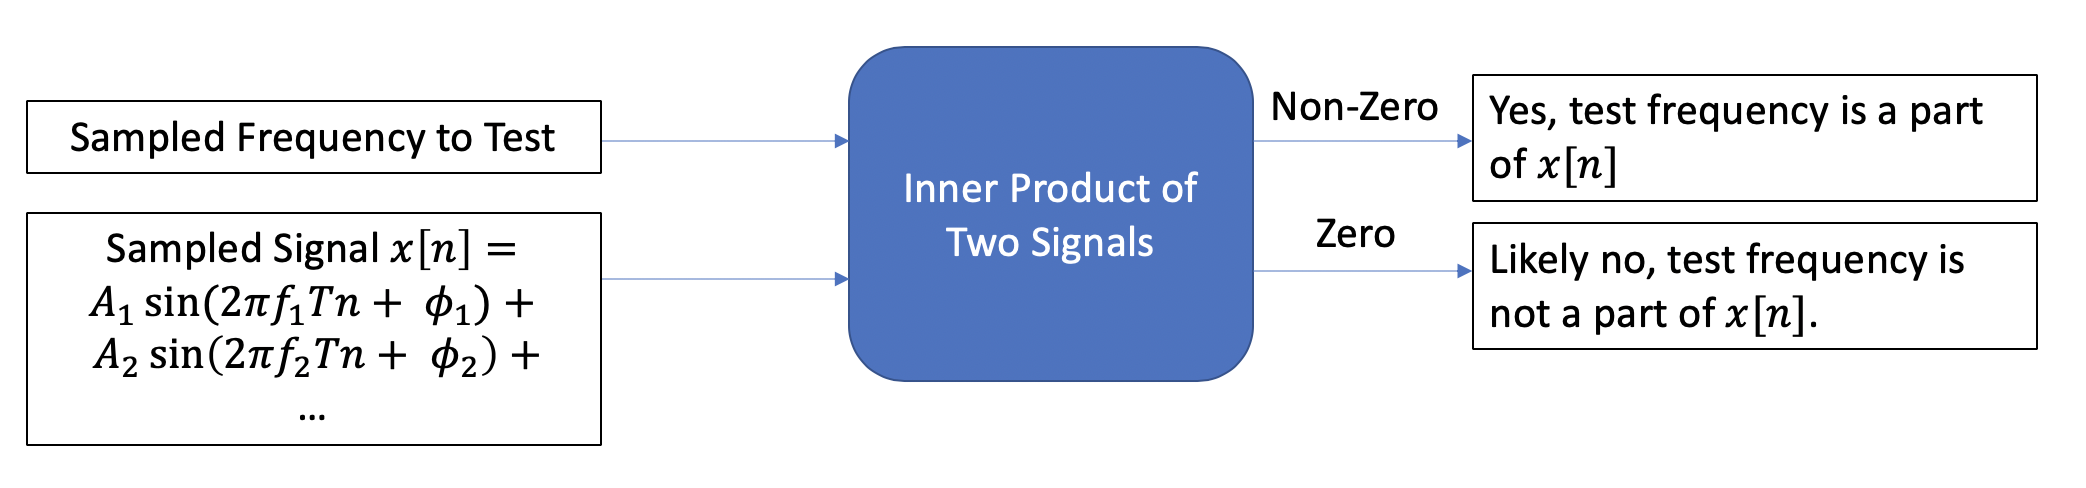
\includegraphics[scale = 0.4]{testImplemented.png}
	\label{fig:testImplemented}
\end{figure}

\noindent Figure \ref{fig:testImplemented} shows an updated version of the behavior of the inner product and what it means.
We can see that a result of zero, \textbf{likely} means that the testing frequency is not part of the audio signal but not
definitively.

How can we ensure that we get a non-zero inner product for sinusoids of the same frequency?  The answer:
take \textbf{two} inner products.  Suppose we have some test frequency and some signal and we would like to 
know whether that test frequency is a part of the signal.  If we take
the inner product between the test frequency and the signal, we run the risk that the answer could be zero even
if the test frequency is a part of the signal.  But if we have two test sinusoids of the same frequency but with
different phases, then at least one of them will yield a non-zero inner product when the audio signal has
that frequency.  

It may not be readibly apparent why using two sinusoids makes any difference.  For simplicity, let us say that
we will test our audio signal using a sine wave and a cosine wave, both of frequency $f_{test}$.  Sine and cosine 
differ in phase by $\pi/2$.  Let us assume that our audio signal also has a component
of frequency $f_{test}$ but we know nothing about that component's phase.  In the original scenario, we would
just take the inner product of our audio signal against a sine wave with frequency $f_{test}$.  Most likely, the
result would be non-zero, successfully indicating the presence of $f_{test}$ in the audio signal.  However,
if the component in the audio signal differs in phase from a sine wave by exactly $\pi/2$, our result would be
zero.  Again, we wish that were not the case.  Notice though that there does not exist any phase that is both 
$\pi/2$ out of phase with both a sine wave \textbf{and} a cosine wave.  Therefore, taking two inner
products, one with sine and one with cosine, ensures that at least one of the results will be non-zero in the
event the frequency is part of the audio signal.  

Figure \ref{fig:testComplete} shows our completed implementation 
of the testing mechanism outlined from
Figure \ref{fig:test}.  Note how we now need two sampled sinusoids: one cosine and one sine.  While this
requires extra processing, we can now definitively conclude the presence of a particularly frequency in an 
audio signal.

\begin{figure}[h]
	\caption{Complete solution for testing frequency components of a signal.}
	\centering
	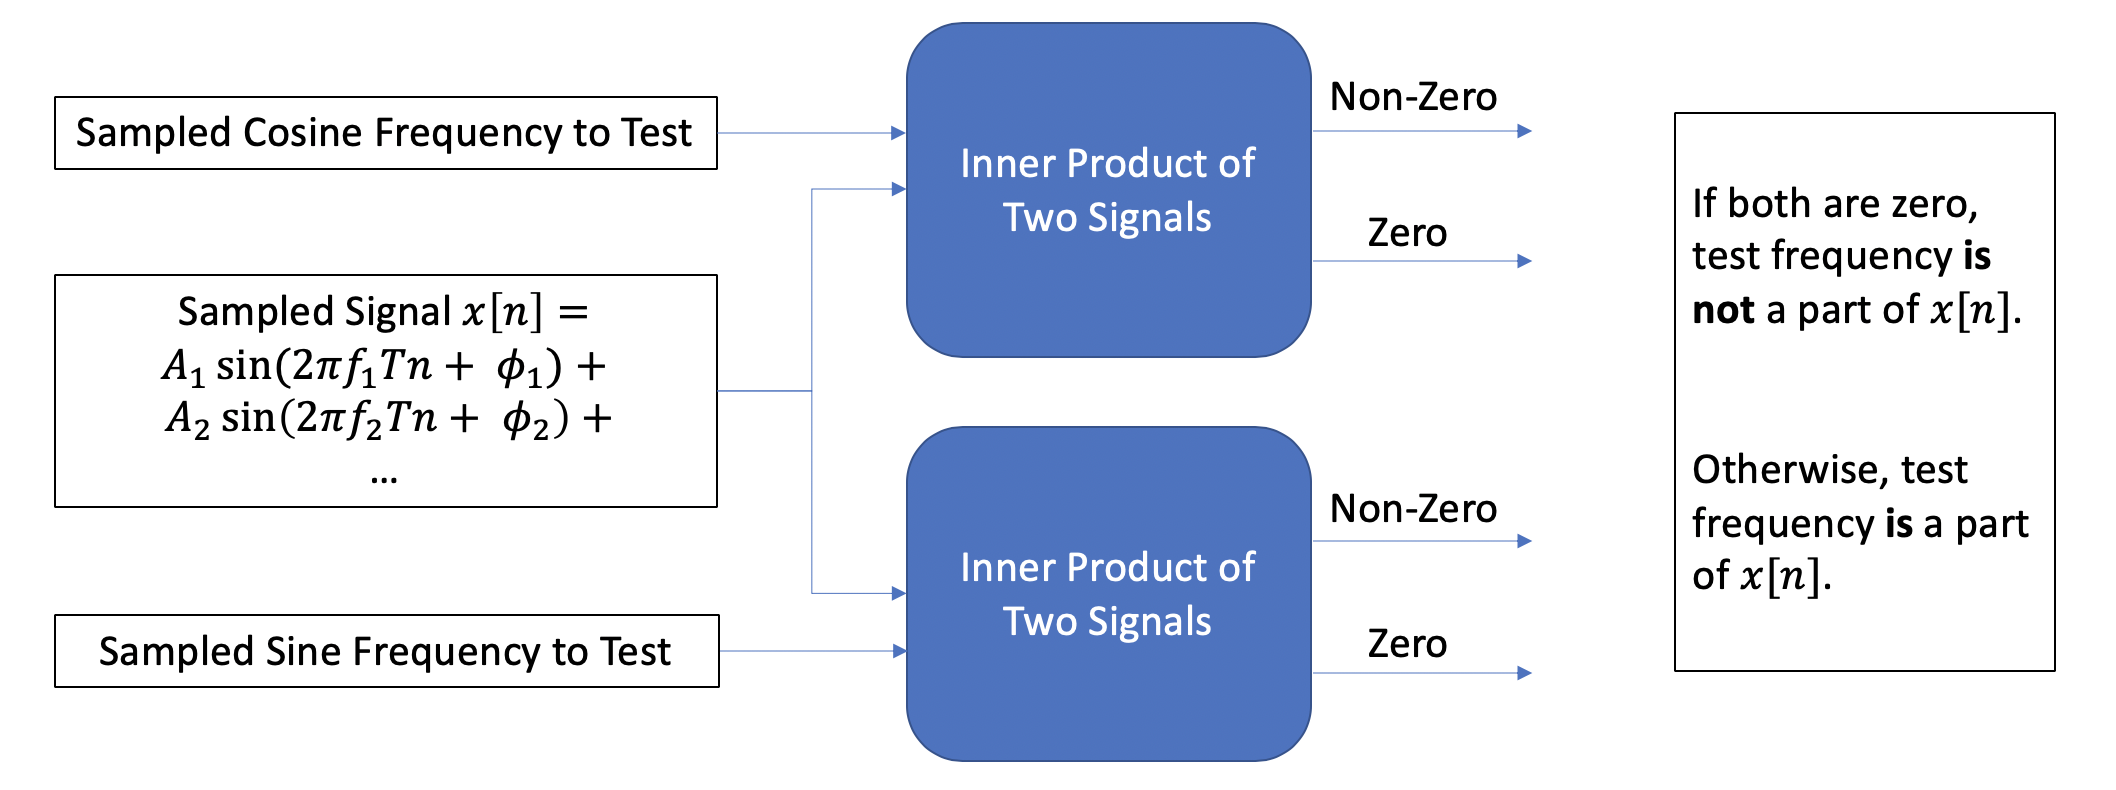
\includegraphics[scale = 0.4]{testComplete.png}
	\label{fig:testComplete}
\end{figure}

The DFT also takes two inner products to determine the presence of a particular frequency.  However, it uses
a cosine wave and a \textbf{negative} sine wave.  The same principles still apply.  There does not exist any
phase that is both $\pi/2$ out of phase with both a cosine and a negative sine wave.  So we will still be able 
to determine the presence of any frequency with certainty.

%If you are curious about how we can prove that $\pi/2$ is an issue, see Appendix B which walks through the math.

\subsection*{Imaginary Numbers}

Figure \ref{fig:testComplete} shows that we will generate two results, one for
each inner product.  In digital signal processing, it is common to hold two separate values in a complex number.  
Perhaps you have encountered complex numbers somewhere in your mathematical training.  Complex numbers
come in the form $a + bi$ where $i$ is called the imaginary unit or number and is defined as $i^2 = -1$.  Already,
this feels perilous on some level.  Why are we using complex numbers for audio signals?  There is nothing
``imaginary" about an audio signal, sine wave, or cosine wave.  So why use them?

In general, complex numbers are important  tools for solving problems in mathematics, engineering and
the physical sciences.  This includes signal processing.  In fact, complex numbers are just as 
``real" as say negative numbers.
It is hard to find a physical analogy to negative numbers.  We cannot pick up $-4$ rocks, for example.  Yet, we 
accept negative numbers because they allow us to work more easily with operations like subtraction.  Complex
numbers are similar.  They are a mathematical tool that allows us to solve problems we would not otherwise be
able to solve.   

When we have a number like $a + bi$, we
separate the real component $a$ from the imaginary component $b$.  The plus sign can be confusing because we cannot actually add $a$ and $b$.  They are treated
as separate and distinct units. It is akin to how coefficients of distinct variables such as $3y + 4z$ cannot be added. 

Because a complex number contains two distinct quantities, the real and imaginary components can be used
to store the results of each inner product.  We can use the real and imaginary components to represent any
two distinct quantities.  For example, we can use complex numbers to represent apples and oranges.  
Perhaps the real component represents the number of apples and the imaginary component represents
the number of oranges.  Then, to express 3 apples and 4 oranges, we can write a single number
$3 + 4i$.  Complex numbers are a convenient device to represent any two distinct values or results.

Complex numbers have another property that makes them the appropriate choice.  The great 
mathematician, Leonhard Euler, discovered one of the fundamental mathematical equations
that relates numbers such as $i$, $e$ as well as $\sin$ and $\cos$.  It is called Euler's formula:

\begin{equation}
\label{eq:euler}
e^{ix} = \cos(x) + i\sin(x)
\end{equation}

This is one of the most remarkable equations in all of mathematics.  The key takeaway is that we can use
a complex exponential to express both a real cosine term and an imaginary sine term.  Again there is
nothing ``imaginary" about the sine wave.  The complex exponential can simply express two 
\textbf{separate} sinusoids.  Fortuitously, a complex exponential is just what we need for our current
problem.  Remember we want to take the inner product of a signal with a cosine and sine wave, and we want to 
keep the results separate.  All we need to do then is to take the inner product of our signal with a complex
exponential.  For example, if we have a signal $x[n]$ and
we want to test it for frequency $f_{test}$, we can compute 

$$\langle x[n], e^{2\pi f_{test}Tni}\rangle =  
\langle x[n], \cos(2\pi f_{test}Tn)\rangle + i\langle x[n], \sin(2\pi f_{test}Tn)\rangle$$  

\noindent This
notation says to take the inner product with the real cosine term of frequency $f_{test}$ and the inner
product with imaginary sine term of frequency $f_{test}$.  Because the real and imaginary numbers are kept
separate, we will get an answer of the form $a + bi$ where $a$ is the result of the inner product with cosine
and $b$ is the result of the inner product with sine. 

\begin{figure}[h]
	\caption{Complete solution using complex exponentials.}
	\centering
	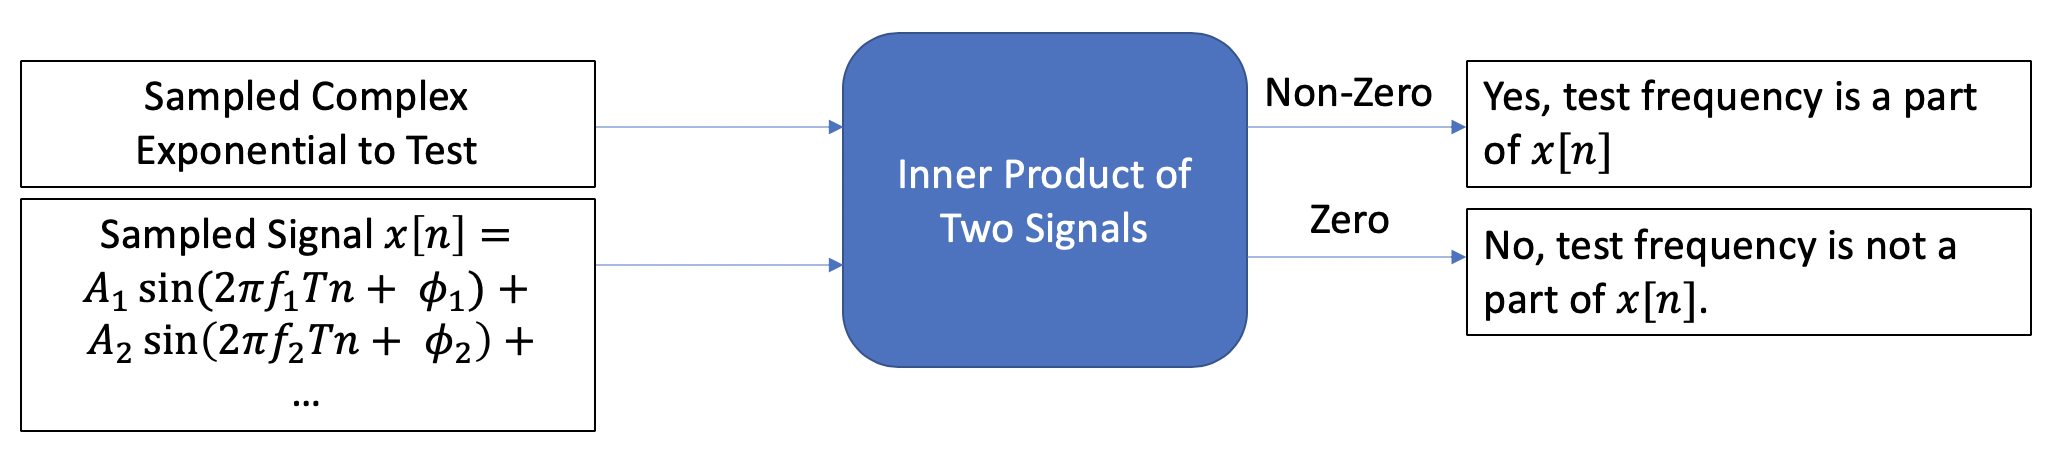
\includegraphics[scale = 0.4]{testComplex.png}
	\label{fig:testComplex}
\end{figure}

Figure \ref{fig:testComplex} shows the updated version of our procedure for calculating the inner product.
It is important to understand that Figure \ref{fig:testComplex} is no different from Figure \ref{fig:testComplete}.  
The inner product in Figure \ref{fig:testComplex} produces two inner products stored in the real and imaginary
components, respectively.  Those are the same inner products calculated in Figure \ref{fig:testComplete}.  If
both the real and imaginary component are zero then we know the test frequency is not a part of our signal
$x[n]$.

As a quick aside, Euler's
formula also allows us to translate back and forth between sinusoids like sine and cosine and exponentials.
Exponentials are much easier to work with and allows us to quickly prove equations like trigonometric identities
that would be much harder if we simply had to work with just sine and cosine.  In general, if you plan to learn
more about digital signal processing, you will need to get comfortable with complex numbers and complex 
exponentials.
